\documentclass[12pt,a4paper]{article}

\usepackage[a4paper,margin=1in]{geometry}
\usepackage{graphicx}
\usepackage{booktabs}
\usepackage{float}
\usepackage{amsmath}
\usepackage{xcolor}
\usepackage{listings}
\usepackage[hidelinks]{hyperref}

\lstset{
  basicstyle=\ttfamily\small,
  columns=fullflexible,
  frame=single,
  breaklines=true,
  showstringspaces=false
}

\title{Packet Error Detection Using Checksums and CRC Schemes}
\author{}
\date{}

\begin{document}

\maketitle
\tableofcontents
\newpage

\section{Introduction}

This project implements a TCP sender and receiver for transmitting a file in
fixed-size packets. Before transmission, each packet receives an integrity
value calculated using one of several error-detection schemes. The receiver
recalculates the selected value and compares it with the value carried in the
packet.

The implemented schemes are:

\begin{itemize}
  \item a 16-bit one's-complement checksum;
  \item CRC-16/CCITT-FALSE, polynomial $0x1021$;
  \item CRC-32/IEEE, reflected polynomial $0xEDB88320$;
  \item CRC-10/ATM, polynomial $0x233$; and
  \item CRC-8/ATM, polynomial $0x07$.
\end{itemize}

The project also contains controlled single-byte and burst-error injection,
an end-to-end evaluator, and Python scripts that produce packet-level tables
and graphs.

\section{Sender and Receiver}

\subsection{Sender responsibilities}

The sender is implemented in \texttt{sender.c}. Its main responsibilities
are establishing a TCP connection, reading the input file, constructing
packets, optionally corrupting them, transmitting all bytes, and receiving
the receiver's final response.

The sender uses \texttt{getaddrinfo()} to obtain address candidates and tries
to create and connect a TCP socket. The default port is 3000, although a
different port can be supplied as a command-line argument. The user selects
an error-injection mode and an error-detection scheme using validated input.

The file is read using:

\begin{lstlisting}[language=C]
while ((bytes_read = fread(buffer, 1, PAYLOADSIZE, file)) > 0) {
    payload = make_packet(buffer, bytes_read, checktype);
    ...
}
\end{lstlisting}

Here, \texttt{PAYLOADSIZE} is 44 bytes. Therefore, each complete file chunk
contains at most 44 data bytes. The final packet may contain fewer bytes;
the length field records the actual number of data bytes.

\subsection{Packet construction}

Every packet has a total size of 64 bytes. Its logical layout is:

\begin{table}[H]
\centering
\begin{tabular}{lll}
\toprule
\textbf{Byte range} & \textbf{Field} & \textbf{Size} \\
\midrule
0--5 & Destination MAC placeholder & 6 bytes \\
6--11 & Source MAC placeholder & 6 bytes \\
12--15 & Combined scheme and payload-length header & 4 bytes \\
16--59 & Payload and zero padding & 44 bytes \\
60--63 & Integrity field & 4 bytes \\
\bottomrule
\end{tabular}
\caption{Packet format used by the sender and receiver.}
\end{table}

The four-byte header is transmitted in network byte order. Its most
significant byte identifies the detection scheme, while the lower 24 bits
contain the payload length:

\begin{lstlisting}[language=C]
header = htonl(((uint32_t)checktype << 24) |
               (uint32_t)payload_len);
\end{lstlisting}

The payload is copied into the 44-byte payload area. Because the packet is
initialised with zeroes, unused bytes in the final packet are padding and do
not contain uninitialised data.

The integrity value is calculated after the packet's first 60 bytes have
been assembled. Error injection occurs after the integrity value is written;
this is essential because the receiver must see a mismatch when the packet
has been changed.

\subsection{Receiver responsibilities}

The receiver is implemented in \texttt{receiver.c}. It creates a listening
socket, binds it to port 3000, calls \texttt{listen()}, and accepts sender
connections. For each connection it repeatedly calls \texttt{recv\_all()}.

TCP is a byte stream and does not preserve application packet boundaries.
Therefore, one call to \texttt{recv()} is not assumed to return a complete
64-byte packet. The helper function keeps receiving until either 64 bytes
have arrived or the sender closes its write side.

After a complete packet is received, the receiver:

\begin{enumerate}
  \item reads and decodes the combined scheme/length header;
  \item rejects invalid scheme identifiers or payload lengths;
  \item selects the checksum, CRC-16, CRC-32, CRC-10, or CRC-8 algorithm;
  \item calculates a new integrity value over the first 60 bytes;
  \item compares the calculated value with the packet's stored value; and
  \item records whether the packet was detected as corrupted.
\end{enumerate}

For evaluation runs, the receiver additionally records the complete received
packet as hexadecimal text, the validation time, and the detection result.
This information is written to the packet-level CSV through the evaluator.

\subsection{TCP termination and deadlock prevention}

After the sender transmits the final packet, it executes:

\begin{lstlisting}[language=C]
shutdown(sockfd, SHUT_WR);
\end{lstlisting}

This is a half-close. It tells the receiver that no more bytes will be sent,
while still allowing the sender to receive data. Consequently,
\texttt{recv\_all()} eventually receives zero from \texttt{recv()}, exits its
receive loop, and the receiver sends its response.

Without this operation, the sender waits for the receiver's response while
the receiver waits for another 64-byte packet. Both processes block
indefinitely.

\section{Error Detection Module}

The algorithms are implemented in \texttt{error\_detection.c} and declared
in \texttt{error\_detection.h}. Each algorithm processes the same protected
60-byte region, which allows the schemes to be compared on the same packet
and the same corruption pattern.

\subsection{One's-complement checksum}

The checksum divides the input into 16-bit words. Each word is interpreted in
big-endian order and added to a running sum. Whenever a carry leaves the
16-bit range, the carry is folded back into the low 16 bits. After all words
are processed, the result is complemented:

\[
S \leftarrow S + W_i
\]

\[
S \leftarrow (S \mathbin{\&} 0xffff) + (S \mathbin{\gg} 16)
\]

\[
\mathrm{checksum} = \mathop{\sim}S.
\]

This is computationally inexpensive, but it is weaker than CRCs for many
structured multi-bit error patterns. Different corruptions can produce the
same one's-complement sum.

\subsection{General CRC operation}

A CRC treats the message as a polynomial over the binary field
$GF(2)$. Addition and subtraction are both XOR operations. The message is
processed bit by bit, and whenever the current register's top bit is set, the
selected generator polynomial is XORed into the shifted register.

The implementation follows this general pattern:

\begin{lstlisting}[language=C]
crc ^= input_byte << register_shift;
for each bit in input_byte:
    if (top_bit_is_set)
        crc = (crc << 1) ^ polynomial;
    else
        crc = crc << 1;
\end{lstlisting}

The polynomial, initial register value, reflection convention, and final XOR
value define a particular CRC variant. These parameters must be identical at
the sender and receiver.

\subsection{CRC-16/CCITT-FALSE}

CRC-16 uses a 16-bit register and generator polynomial $0x1021$. The
implementation uses initial value $0xffff$, non-reflected input and output,
and final XOR value zero. For each input byte, the byte is shifted into the
upper eight bits of the register. Eight iterations then process the byte.

The resulting 16-bit value is stored in the final two bytes of the packet's
integrity field. The first two bytes of that field are zero.

\subsection{CRC-32/IEEE}

CRC-32 uses a 32-bit register. The implementation uses the reflected IEEE
polynomial $0xEDB88320$, initial value $0xffffffff$, reflected processing, and
final XOR value $0xffffffff$.

Because CRC-32 produces four bytes, it occupies the complete integrity field
at bytes 60--63. The receiver reconstructs the 32-bit received value in
big-endian order before comparing it with its calculated value.

\subsection{CRC-10/ATM}

CRC-10 uses a 10-bit register and polynomial $0x233$. Its initial value and
final XOR value are zero, with non-reflected processing. The calculated value
is limited to 10 bits and stored in the final two bytes of the integrity
field.

\subsection{CRC-8/ATM}

CRC-8 uses an 8-bit register and polynomial $0x07$, with initial value zero,
non-reflected processing, and final XOR value zero. The eight-bit result is
stored in byte 63 of the integrity field; bytes 60--62 are zero for this
scheme.

Compared with larger CRCs, CRC-8 has a smaller result space and therefore a
higher probability of undetected collisions for sufficiently large or
structured error sets. However, it is computationally inexpensive and can
detect many common short errors.

\section{Error Creation}

Error creation is implemented in \texttt{error\_injection.c}. The module
supports three modes:

\begin{itemize}
  \item no error;
  \item a single-byte error, implemented by XORing one byte with 1 at a
        selected packet position; and
  \item a burst error, implemented by XORing consecutive packet bytes with 1.
\end{itemize}

For reproducible comparisons, the evaluator assigns one seed to each test
case. The same seed, error mode, burst length, and input file are then used
for every detection scheme. Consequently, a row in the packet comparison
table compares schemes against the same corrupted packet rather than against
independently random errors.

The sender records the actual start position and length of each injected
error. The receiver records the complete received packet, so the resulting
failure report identifies both the corruption location and the packet bytes.

\section{Experimental Evaluation}

The experiment used the real sender and receiver processes. The evaluator
ran the schemes on packets containing different error types and collected:

\begin{itemize}
  \item whether each scheme detected each packet error;
  \item the exact packet index and error byte range;
  \item the full received packet in hexadecimal form;
  \item validation time measured by the receiver;
  \item sender wall-clock time and CPU usage; and
  \item memory usage and invalid-metadata detections.
\end{itemize}

The experiment was performed over 1,000 packet trials with clean, single-bit,
and burst-error cases. The same error instance was presented to every scheme
in a comparison group. The packet-level output identifies the schemes that
succeeded and failed for each exact error.

\subsection{Validation time}

Figure~\ref{fig:validation-time} shows the distribution of receiver
validation times. The boxplot displays the median, interquartile range, and
variation of the measured time for each scheme. A larger CRC register and a
more computationally involved bit-processing loop generally require more
operations than the one's-complement checksum. The measured values should be
interpreted as implementation-level measurements on the test machine; they
are not universal hardware-independent constants.

\begin{figure}[H]
  \centering
  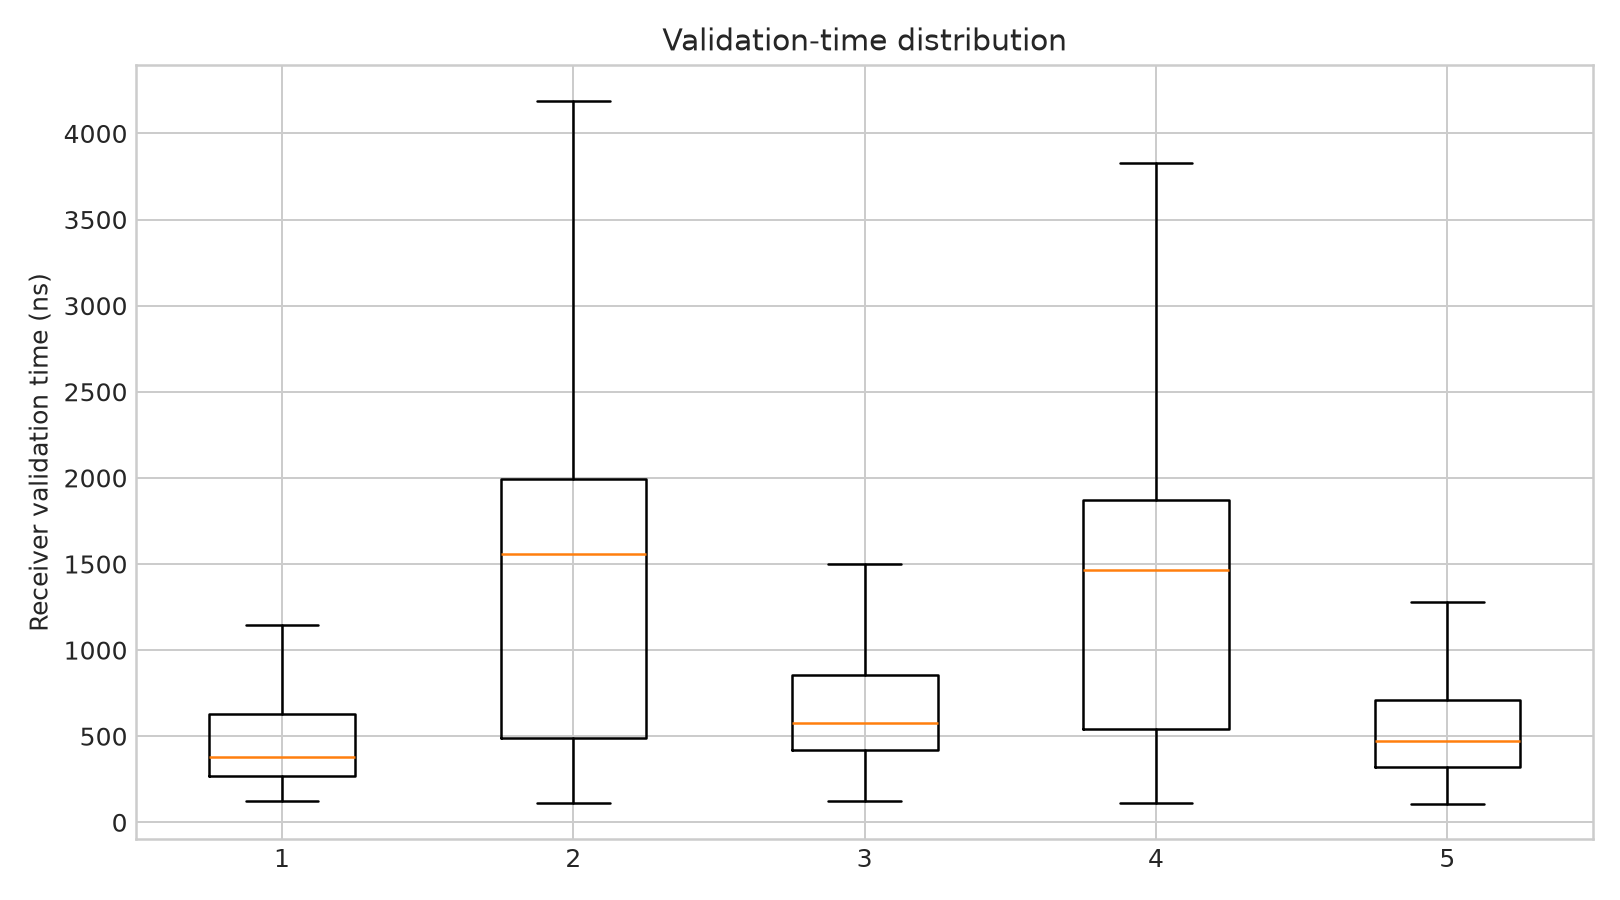
\includegraphics[width=0.88\textwidth]{validation_time_boxplot.png}
  \caption{Receiver validation-time distribution for the detection schemes.}
  \label{fig:validation-time}
\end{figure}

\subsection{Scheme failures}

Figure~\ref{fig:scheme-failures} shows the number of packet errors missed by
each scheme. A failure means that the received packet was corrupted but the
scheme's calculated value still matched the stored value. The corresponding
failure-only files provide the exact evidence for each bar:
\texttt{failed\_packets.csv} contains the structured records and
\texttt{failed\_packets\_report.txt} contains the packet hexadecimal data,
error range, successful schemes, failed schemes, and per-scheme validation
times.

\begin{figure}[H]
  \centering
  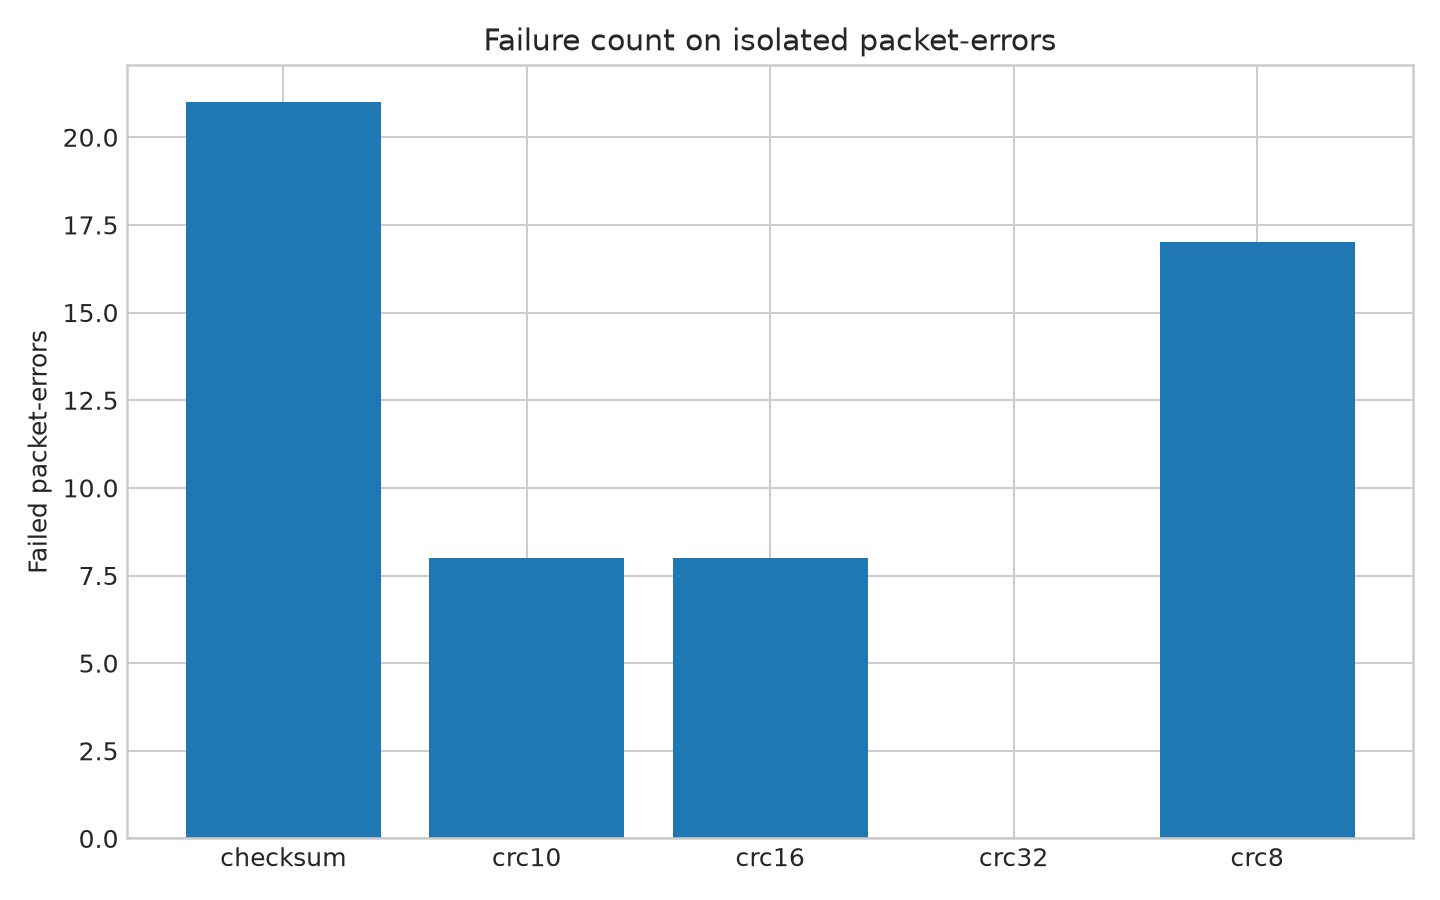
\includegraphics[width=0.82\textwidth]{failed_packets_by_scheme.png}
  \caption{Number of error packets missed by each scheme.}
  \label{fig:scheme-failures}
\end{figure}

\section{Conclusion}

The implementation separates packet transport from integrity validation. The
sender constructs fixed-size packets and transmits them over TCP, while the
receiver reconstructs the packet and applies the scheme selected in the
packet header. The checksum is simple and fast, whereas CRCs provide stronger
polynomial error detection with different computation costs and result
widths.

The reproducible end-to-end evaluator makes the comparison packet-specific:
the exact same corrupted packet is tested by every scheme. Therefore, the
failure report can answer the central experimental question directly: for a
particular packet and error range, which schemes detected the error and which
ones failed to detect it.

\end{document}
